\section{Auswertung}
<<<<<<< HEAD
\label{sec:auswertung}
Es werden in diesem Versuch zwei Messreihen mit unterschiedlicher Heizrate
$b$ durchgeführt. Zunächst müssen die Messwerte von Untergründen bereinigt
werden, auf die im Folgenden eingegangen wird.
Für die erste Messreihe -- im Folgenden mit dem Index A gekennzeichnet --
gilt $b_\text{A} = \SI{2}{\kelvin\per\minute}$, für die Zweite, mit B
gekennzeichnete Messreihe gilt $b_\text{B} = \SI{4}{\kelvin\per\minute}$.

Alle Fehler in dieser Auswertung werden -- wenn nicht anders beschrieben --
mittels Gaußscher Fehlerfortpflanzungen mit Hilfe des \texttt{python}-Paketes
\texttt{uncertainties} \cite{py-uncertainties} berechnet.

Zur Beschreibung des oben genannten Untergrundes wird bei Messreihe A eine
exponentielle Funktion $I_\text{bkg,A}(T)$ und bei Messreihe B eine lineare
Funktion
$I_\text{bkg,B}(T)$ von den Daten abgezogen. Die Variablen der Funktionen werden
durch Fit an einen Teil der Daten bestimmt, der in Abbildungen
\ref{fig:data-a} und \ref{fig:data-b} markiert ist.
Die Fitfunktionen haben die Gestalt
\begin{align*}
    I_\text{bkg,A}(T) &= A_1 e^{B_1 (T-T_0)} + C_1\,,\\
    I_\text{bkg,B}(T) &= A_2\cdot T + B_2\,.
\end{align*}
Das Resultat, sowie der Fit sind ebenfalls in oben genannter Abbildung
dargestellt und die entsprechenden Daten in den Tabellen \ref{tab:data1} und
\ref{tab:data2} aufgeführt.
Im weiteren Verlauf wird dabei jeweils ein offset $I_\text{off}$ von den Daten
abgezogen. Dieser beträgt für Datensatz A $I_\text{off} = \SI{1.46}{\pico\ampere}$
und für Datensatz B $I_\text{off} = \SI{8.1}{\pico\ampere}$.
\begin{figure}
    \centering
    \includegraphics[width=0.8\linewidth]{build/plots/cleaned_data-set1.pdf}
    \caption{Messdaten der Messreihe A, roh und bereinigt.}
    \label{fig:data-a}
\end{figure}
\begin{figure}
    \centering
    \includegraphics[width=0.8\linewidth]{build/plots/cleaned_data-set2.pdf}
    \caption{Messdaten der Messreihe B, roh und bereinigt. Hier ist
    der zu erwartende Peak gut zu erkennen.}
    \label{fig:data-b}
\end{figure}
\begin{table}
    \centering
    \caption{Messdaten von Messreihe A mit Heizrate $b = \SI{2}{\kelvin\per\minute}$.}
    \label{tab:data1}
    \input{data/data-set1.tex}
\end{table}
\begin{table}
    \centering
    \caption{Messdaten von Messreihe B mit Heizrate $b = \SI{4}{\kelvin\per\minute}$.}
    \label{tab:data2}
    \input{data/data-set2.tex}
\end{table}
Bei der ersten Messreihe ist auffällig, dass nur ein einzelner, flacher Peak
zu erkennen ist. Dies macht die spätere Auswertung extrem schwierig.
Aus diesem Grund werden die Ergebnisse der erste Messreihe im weiteren
Verlauf nicht betrachtet.

\subsection{Approximative Ausgleichsrechnung}
\label{subsec:approx}
Zunächst wird die in Abschnitt \ref{sub:berechnung_der_aktivierungsenergie_w_}
aufgeführte Gleichung \ref{eqn:approx} zur Bestimmung der Aktivierungsenergie
$W$ benutzt. Dabei wird diese mit einem nicht-linearen Fit in einem Bereich
$T$ zwischen \SIrange{250}{267}{\kelvin} an die Daten angepasst.
Das Ergebnis des Fits ist in Abbildung \ref{fig:fit_approx_set2} dargestellt.
Der Fit liefert von Messreihe A liefert
\begin{equation*}
    \input{build/tex/W_approx_set1.tex}\,,
\end{equation*}
das entsprechende Ergebnis aus Messreihe B liefert
\begin{equation*}
    \input{build/tex/W_approx_set2.tex}\,.
\end{equation*}
Die zugehörigen Fits sind in Abbildungen \ref{fig:fit_approx_set1}
und \ref{fig:fit_approx_set2} dargestellt.
\begin{figure}
    \centering
    \includegraphics[width=0.8\linewidth]{build/plots/fit_approx_set1.pdf}
    \caption{Ausgleichskurve zur approximativen Bestimmung der
    Aktivierungsenergie $W$ mit Datensatz A. Die für den Fit benutzten Datenpunkte
    sind grün markiert.}
    \label{fig:fit_approx_set1}
\end{figure}
\begin{figure}
    \centering
    \includegraphics[width=0.8\linewidth]{build/plots/fit_approx_set2.pdf}
    \caption{Ausgleichskurve zur approximativen Bestimmung der
    Aktivierungsenergie $W$ mit Datensatz B. Die für den Fit benutzten Datenpunkte
    sind grün markiert.}
    \label{fig:fit_approx_set2}
\end{figure}

\subsection{Ausgleichsrechnung mit Integration}
\label{subsec:integration}
Als zweite Methode zur Bestimmung der Aktivierungsenergie $W$ wird ein
linearer Fit der Form
\begin{equation*}
    F(T) = \alpha\cdot\frac{1}{T} + \beta
\end{equation*}
an die inversen Temperaturdaten $1/T$ durchgeführt.
Hierbei ist $F(T)$ wie in Gleichung \ref{eqn:integrate} definiert als
\begin{equation*}
    F(T) = \frac{\int_T^{T^\ast} i(T^\prime)\mathrm{d}T^\prime}{i(T)}\,.
\end{equation*}
Aus der Steigung $A$ lässt sich somit die Aktivierungsenergie $W$
berechnen durch
\begin{equation*}
    W = \alpha\cdot k_\text{B}\,.
\end{equation*}
Außerdem wird schließlich die Relaxationszeit $\tau_0$ aus der Temperatur
bei maximalem Strom $T_\text{max}$ bestimmt:
\begin{equation}
    \label{eqn:tau0}
    \tau_0 = \frac{k_\text{B}T_\text{max}^2}{Wb}
             \exp\!\left[-\frac{W}{k_\text{B}T_\text{max}} \right]
\end{equation}
Die Fits sind in Abbildungen \ref{fig:integrate_fit1} und \ref{fig:integrate_fit2}
dargestellt, sie liefern
\begin{equation*}
    \input{build/tex/W_integrated_set1.tex} \qquad\text{und}\qquad \input{build/tex/tau0_integrated_set1.tex}
\end{equation*}
für Datensatz A in einem Bereich $T \in [\SI{260}{\kelvin}, \SI{310}{\kelvin}]$ bei $\input{build/tex/T_max_set1.tex}$ und
\begin{equation*}
    \input{build/tex/W_integrated_set2.tex} \qquad\text{und}\qquad \input{build/tex/tau0_integrated_set2.tex}
\end{equation*}
für Datensatz B in einem Bereich $T \in [\SI{250}{\kelvin}, \SI{280}{\kelvin}]$ bei $\input{build/tex/T_max_set2.tex}$.
Die Fehler dieser Werte berücksichtigen jedoch keine systematischen Unsicherheiten
und werden daher stark unterschätzt. Darauf wird in der Diskussion weiter eingegangen.
\begin{figure}
    \centering
    \includegraphics[width=0.9\linewidth]{build/plots/integrated-fit-set1.pdf}
    \caption{Fit an linearisierte Daten von Messung A.}
    \label{fig:integrate_fit1}
\end{figure}
\begin{figure}
    \centering
    \includegraphics[width=0.9\linewidth]{build/plots/integrated-fit-set2.pdf}
    \caption{Fit an linearisierte Daten von Messung B.}
    \label{fig:integrate_fit2}
\end{figure}

\newpage
\section{Diskussion}
\label{sec:diskussion}
Alle hier durchgeführten Methoden zur Bestimmung der Aktivierungsenergie $W$
liefern Werte im erwarteten Bereich von einigen Millielektronvolt.
Die verschiedenen Messreihen liefern unterscheiden sich jedoch um einen Faktor
\input{build/tex/W_ratio_approx.tex} (approximative Methode) beziehungsweise
\input{build/tex/W_ratio_integrated.tex} (integrierende Methode), was
auf systematische Fehler hindeutet und mit weiteren Messungen untersucht
werden muss.

Die mit Hilfe der integrierenden Methode bestimmten Werte der Relaxationszeit
$\tau_0$ sind schließlich nicht signifikant.
Die Fehler berücksichtigen nicht die starke Abhängigkeit von $\tau_0$ von der
Aktivierungsenergie $W$, die in Abbildung \ref{fig:_tau_test} dargestellt ist.
Bei einer Änderung von $W$ um einige \SI{100}{\milli\electronvolt} ändert
sich der Wert der Relaxationszeit bereits um etliche Größenordnungen.
Änderungen in diesem Bereich treten bereits auf, wenn der Wertebereich des Fits
leicht verändert wird und einige Meßpunkte mehr oder weniger betrachtet werden.
Die damit verbundenen Fehler machen eine Aussage über den wahren Wert von
$\tau_0$ unmöglich.
Die Unsicherheit $\Delta\tau_0$ sollte daher wesentlich zu größeren Werten hin
korrigiert werden.
\begin{figure}
    \centering
    \includegraphics[width=0.8\linewidth]{build/plots/_tau0_test.pdf}
    \caption{Relaxationszeit $\tau_0$ (Gleichung \ref{eqn:tau0}) in Abhängigkeit der Aktivierugnsenergie $W$.}
    \label{fig:_tau_test}
\end{figure}
||||||| d0ac902
\label{sec:Auswertung}

\begin{figure}
  \centering
  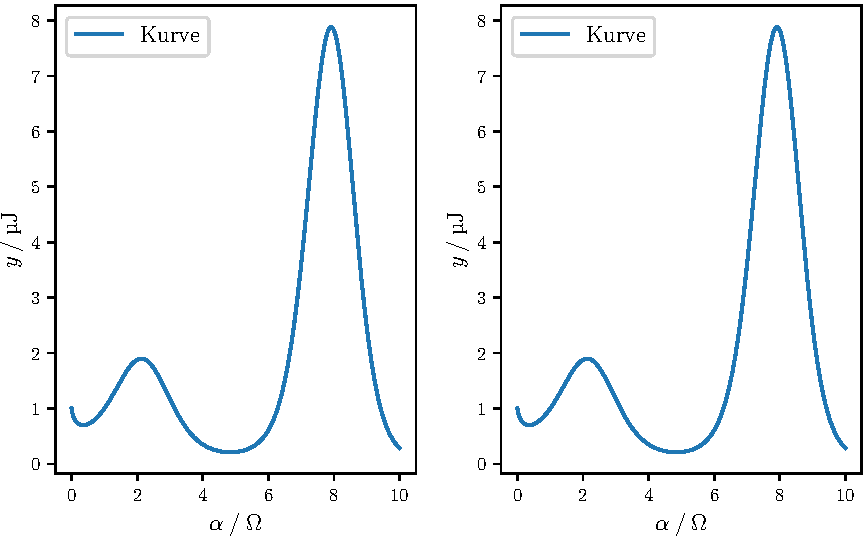
\includegraphics{plot.pdf}
  \caption{Plot.}
  \label{fig:plot}
\end{figure}
=======
\label{sec:Auswertung}
>>>>>>> 70a2a2a488088ae84a88e83b545bba50fc84320c
